\documentclass[t]{beamer}
\setbeameroption{show notes}
%hide all notes
%\setbeameroption{hide notes}

% German style date formatting (footer)
\usepackage[ddmmyyyy]{datetime}
\renewcommand{\dateseparator}{.}

% Format the captions used for figures etc.
\usepackage[compatibility=false]{caption}
\captionsetup{singlelinecheck=off,justification=raggedleft,labelformat=empty,labelsep=none}



\usepackage{etex} % cures ``No room for a new \dimen'' error

%%%%%% font size handling %%%%%%
\RequirePackage{fix-cm}
\usepackage{lmodern}
\DeclareFontFamily{OMX}{lmex}{} % proper math mode size (http://tex.stackexchange.com/questions/74623/big-integral-in-lmodern)
\DeclareFontShape{OMX}{lmex}{m}{n}{<-> lmex10}{}
% \addtokomafont{disposition}{\rmfamily}

%%%%%% better enumerate environment
\usepackage{enumitem}

%%%%%% bold math %%%%% (boldsymbol)
\usepackage{bm}

%%%%%% textdegree %%%%%
\usepackage{ textcomp }

%%%%%% tikz %%%%%%
% \usepackage{pdfpages}
\usepackage{pgfplots}
\pgfplotsset{compat=newest}
\usepackage{tikz}
\usetikzlibrary{fit}

\usetikzlibrary{arrows}
\usetikzlibrary{arrows.meta} % propper scaling of arrows
\pgfplotsset{plot coordinates/math parser=false}
\usetikzlibrary{plotmarks}
% \usetikzlibrary{decorations.shapes}
% \usetikzlibrary{decorations.pathmorphing}
\usepgfplotslibrary{fillbetween}
\usetikzlibrary{patterns}
\usetikzlibrary{intersections}
% \usetikzlibrary{decorations.markings}
% \usetikzlibrary{arrows.meta}
\usepackage{graphicx}
\usepackage{amssymb}
\usepackage{multimedia}
\usepackage{array}
\usepackage{booktabs,adjustbox}
\usepackage{marvosym}
\usepackage{hyperref}
\usetikzlibrary{calc}
% \usepackage{animate}
% \usepackage{movie15}
\usepackage{pdfpages}
\usepackage{pifont}
\newcommand{\cmark}{\ding{51}}%
\usepackage[thinlines]{easytable}

%%%%%% additional packages %%%%%%
% \usepackage{wrapfig}
\usepackage[absolute,overlay]{textpos}
\usetikzlibrary{positioning}
\usepackage{arydshln}
\usepackage{setspace}
\usepackage{multirow}
\usepackage{multicol}
\usepackage{import}
\usepackage{mathtools}

\usepackage{diagbox}
\usetikzlibrary{matrix}


%%%%%% plot sizes %%%%%%
\def\plottitlefontsize{\Large}
\def\plotlabelfontsize{\normalsize}
\def\plotlegendfontsize{\scriptsize}
\def\plottickfontsize{\normalsize}
% \def\plottickfontsize{\tiny}
\def\plotlinewidth{1pt}
\def\plotnodefontsize{\small}

\newlength\figureheight
\newlength\figurewidth

%%%%%% triangles as item markers %%%%%%
\setlist[itemize,1]{label={\small\raise2.5pt\hbox{\donotcoloroutermaths{\color{rwth-75}$\blacktriangleright$}}}}
\setlist[itemize,2]{label={\small\raise2.5pt\hbox{\donotcoloroutermaths{\color{rwth}$\triangleright$}}}}




 \usepackage{pdfpages}
%%%%%% a footnote box for references %%%%%%
\newcounter{grcitenumber}
\newcommand{\declcite}[1]{\refstepcounter{grcitenumber}\label{#1}}
% \newcommand{\showcite}[1]{\ensuremath{\grm{^{\mathit{[\ref{#1}]}}}}}
\newcommand{\showcite}[1]{\ensuremath{\grm{^{\mathit{[#1]}}}}}
% % \newcommand{\greycite}{\stepcounter{grcitenumber}{\ensuremath{\bm{^{\mathit{[\thegrcitenumber]}}}}}}
\newcommand{\citetext}[2]{\grm{$\mathit{[#1]:}$\ \textit{#2}}}
\newcommand{\showlargecite}[1]{\grm{$\mathit{[#1]}$}}
\newcommand{\citebox}[2]{\begin{textblock*}{\textwidth}(0.8cm,16.2cm)\setstretch{0.5}\citetext{#1}{#2}\end{textblock*}}
\newcommand{\citeboxx}[4]{\begin{textblock*}{\textwidth}(0.8cm,15.7cm)\setstretch{0.5}\citetext{#1}{#2} \\ \citetext{#3}{#4}  \end{textblock*}}
\newcommand{\citeboxxx}[6]{\begin{textblock*}{\textwidth}(0.8cm,15.2cm)\setstretch{0.5}\citetext{#1}{#2} \\ \citetext{#3}{#4} \\ \citetext{#5}{#6} \end{textblock*}}
\newcommand{\citeboxxxx}[8]{\begin{textblock*}{\textwidth}(0.8cm,14.7cm)\setstretch{0.5}\citetext{#1}{#2} \\ \citetext{#3}{#4} \\ \citetext{#5}{#6} \\ \citetext{#7}{#8} \end{textblock*}}

\def\grm#1{\color{black-75}{#1}\color{black}}
%%%%% theorems %%%%%%
\newtheorem{remark}[theorem]{Remark}

%%%%%% backup slides not counting to page numbers %%%%%%
\newcommand{\backupbegin}{
   \newcounter{finalframe}
   \setcounter{finalframe}{\value{framenumber}}
}
\newcommand{\backupend}{
   \setcounter{framenumber}{\value{finalframe}}
}

%%%%% custom commands %%%%%%
\def\rhf#1{#1 \rfloor} 
\def\prhf#1#2{#1 \rfloor_{#2}} 
\def\lhf#1{\lceil #1}
\def\plhf#1#2{\lceil^{#2} #1}
\def\mean#1{\langle #1 \rangle}
\def\ns#1{\underline{#1}}
\def\ssum#1{\sum_{\substack{#1}}}
\def\sprod#1{\prod_{\substack{#1}}}
\def\ltimes{\times \ldots \times}
\def\lotimes{\otimes \ldots \otimes}
\def\tr#1{{#1}^T}
\def\sp#1#2{\langle #1,#2 \rangle}
\def\sm#1{\mbox{\large\boldmath$($} #1 \mbox{\large\boldmath$)$}}
\def\mean#1{\langle #1 \rangle}
\def\q#1{``#1``}
\def\lhb#1{\mathcal{L}(#1)} 
\def\rhb#1{\mathcal{R}(#1)}

\newcommand{\diver}{\mathop{\rm div}}
\newcommand{\Ind}{\mathcal{I}}
\newcommand{\Index}{\mathcal{I}}
\newcommand{\K}{\ensuremath{\mathbb{K}}}
\newcommand{\R}{\ensuremath{\mathbb{R}}}
\newcommand{\C}{\ensuremath{\mathbb{C}}}
\newcommand{\N}{\ensuremath{\mathbb{N}}}
\newcommand{\Z}{\ensuremath{\mathbb{Z}}}
% \newcommand{\argmin}{\mathop{\rm argmin}}
\DeclareMathOperator*{\argmin}{argmin}
\newcommand*\intd{\mathop{}\!\mathrm{d}}







\usetheme{rwth}

% Setup presentation information
\title{Training DNNs in Low-Dimensional Subspaces}
\subtitle{Master Colloquium $|$ Janik Philipps}
\date[RWTH]{Master Colloquium \enskip|\enskip\today}
\author[Max]{Janik Philipps}
\institute[RWTH]{RWTH Aachen}

\logo{
\includegraphics{logo}}

\include{stmaryrd}

\usepackage{amsthm}
\usepackage{amssymb}
\renewcommand{\N}{\mathbb{N}}
\renewcommand{\R}{\mathbb{R}}	
\newcommand{\A}{\mathcal{A}}
\newcommand{\B}{\mathcal{B}}
\newcommand{\D}{\mathcal{D}}
\newcommand{\F}{\mathcal{F}}
\newcommand{\I}{\mathcal{I}}
\newcommand{\X}{\mathcal{X}}
\newcommand{\Y}{\mathcal{Y}}
\renewcommand{\O}{\mathcal{O}}
\renewcommand{\H}{\mathcal{H}}
\renewcommand{\L}{\mathcal{L}}
\renewcommand{\P}{\mathcal{P}}

\renewcommand{\b}{\mathsf{b}}
\newcommand{\w}{\mathsf{w}}
\renewcommand*{\tr}{^{\mkern-1.5mu\mathsf{T}}}

\usepackage{amsmath}
\DeclareMathOperator*{\E}{\mathbb{E}}

\begin{document}

\definecolor{def_color}		{RGB}{0,84,159}
\definecolor{def_shade_color}	{RGB}{199,221,242}
\definecolor{def_title_color}	{RGB}{0,84,159}
\definecolor{def_frame_color}	{RGB}{64,127,183}

\definecolor{thm_shade_color}	{RGB}{254,234,201}	
\definecolor{thm_title_color}	{RGB}{0,0,0}
\definecolor{thm_frame_color}	{RGB}{250,190,80}

\setbeamercolor{title page bar}{fg=white}
\setbeamertemplate{title page}[rwth][title_small]{}


\setbeamercolor{block title}{bg=def_frame_color, fg=white}
\setbeamercolor{block body}{bg=def_shade_color, fg=black}
\setbeamercolor{block title alerted}{bg=thm_frame_color, fg=white}
\setbeamercolor{block body alerted}{bg=thm_shade_color, fg=black}



%%%%%%%%%%%%%%%%%%%%%%%%%%%%%%%%%%%%%%%%%%%%%%%%%%%%%%%%%%%%%%%

\begin{frame}[plain]
\titlepage
\end{frame}

%%%%%%%%%%%%%%%%%%%%%%%%%%%%%%%%%%%%%%%%%%%%%%%%%%%%%%%%%%%%%%%

\section{Motivation 1/2: Deep neural networks depend on million of parameters causing severe problems.}
\begin{frame}
\begin{columns}[c]

\begin{column}{0.4\textwidth}
\begin{center}
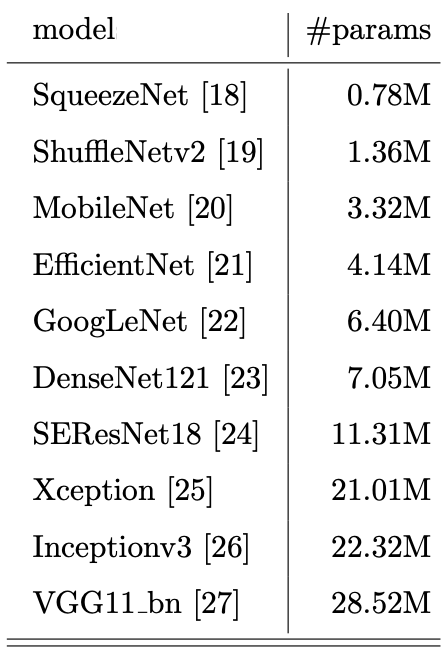
\includegraphics[width=0.92\textwidth]{parameters.png}
\end{center}
\end{column}

\begin{column}{0.5\textwidth}
\begin{itemize}
\item Potential overfitting of the data \vspace{1cm}
\item Computationally and time intensive training \vspace{1cm} 
\item Many training data needed \vspace{1cm}
\item Questionable solution quality  
\end{itemize}
\end{column}

\end{columns}
\end{frame}



\section{Motivation 2/2: The number of independent optimization variables may be smaller than the number of parameters.}
\begin{frame}
\begin{itemize}
\item Due to strong mutual relationships, \textbf{regarding each parameter} of deep neural networks \textbf{as an independent variable is too rough}. \vspace{0.3cm}
\item The \textbf{gradients of parameters are strongly related} due to the training via backpropagation. \vspace{0.4cm}
\item The parameters in the same layers also have \textbf{synergy correlations}. \vspace{0.8cm}
\end{itemize}
\center{$\Downarrow$} \vspace{0.8cm}
\begin{center}
\fbox{\parbox[c]{23cm}{\textbf{The Low-Dimensonal Trajectory Hypothesis:} \\ For a neural network with $n$ parameters, the parameters' trajectory over training can be approximately covered by a $d$-dimensional space with $d \ll n$. [1]}}
\end{center}
\end{frame}



%\section{The Low-Dimensional Trajectory Hypothesis}
%\begin{frame}
%\begin{center}
%\parbox{23cm}{\center ''For a neural network with $n$ parameters, the parameters' trajectory over training can be approximately covered by a d-dimensional space with $d \ll n$.`` [1]}
%\end{center}

%\vspace{5cm}
%[1] Tao Li, Lei Tan, Qinghua Tao, Yipeng Liu, Xiaolin Huang. \textit{Low Dimensional Trajectory Hypothesis is True: DNNs can be Trained in Tiny Subspaces}. IEEE Transactions on Pattern Analysis and Machine Intelligence, 2022.
%\end{frame}


%\section{Motivation: Pioneering work achieved 90\% accuracy in smaller spaces}
%\begin{frame}
%\begin{itemize}
%\item There exists pioneering work on \textbf{training via random projections} \vspace{1cm}
%\item For example, on CIFAR-10, LeNet with 62006 parameters could be optimized in 2900-dimensional subspaces with 
%\textbf{90\% accuracy of regular SGD training}. \vspace{1cm}
%\center{$\downarrow$} \vspace{1cm}
%\center{Very promising but we can do even better!} \vspace{1cm}
%\item{Many standard neural network architectures could be \textbf{well trained by only 40 independent variables} with almost the same performance. }
%\end{itemize}
%\end{frame}

\section{Illustration of the low-dimensional trajectory hypothesis}
\begin{frame}
\begin{columns}[c]

\begin{column}{0.5\textwidth}
\begin{center}
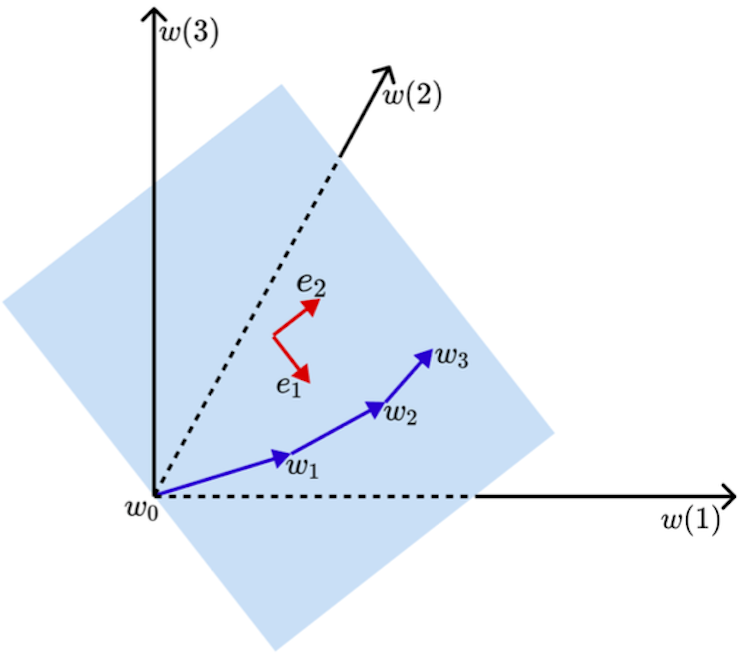
\includegraphics[width=0.99\textwidth]{approach.png}
\end{center}
\end{column}

\begin{column}{0.5\textwidth}
\begin{itemize}
\item There are \textbf{three parameters} $w(1)$, $w(2)$, $w(3)$ \textbf{to optimize}. \vspace{1cm}
\item The training trajectory $\{w_i\}_{i=0,\dots,t}$ could be in a \textbf{two-dimensional subspace} spanned by $e_1$ and $e_2$. \vspace{1cm} 
\item Training in the low-dimensional space can have \textbf{comparable performance} as training in the regular space.
\end{itemize}
\end{column}
\end{columns}
\end{frame}



\section{Agenda}
\begin{frame}
\begin{columns}[c]

\begin{column}{0.5\textwidth}
\begin{center}
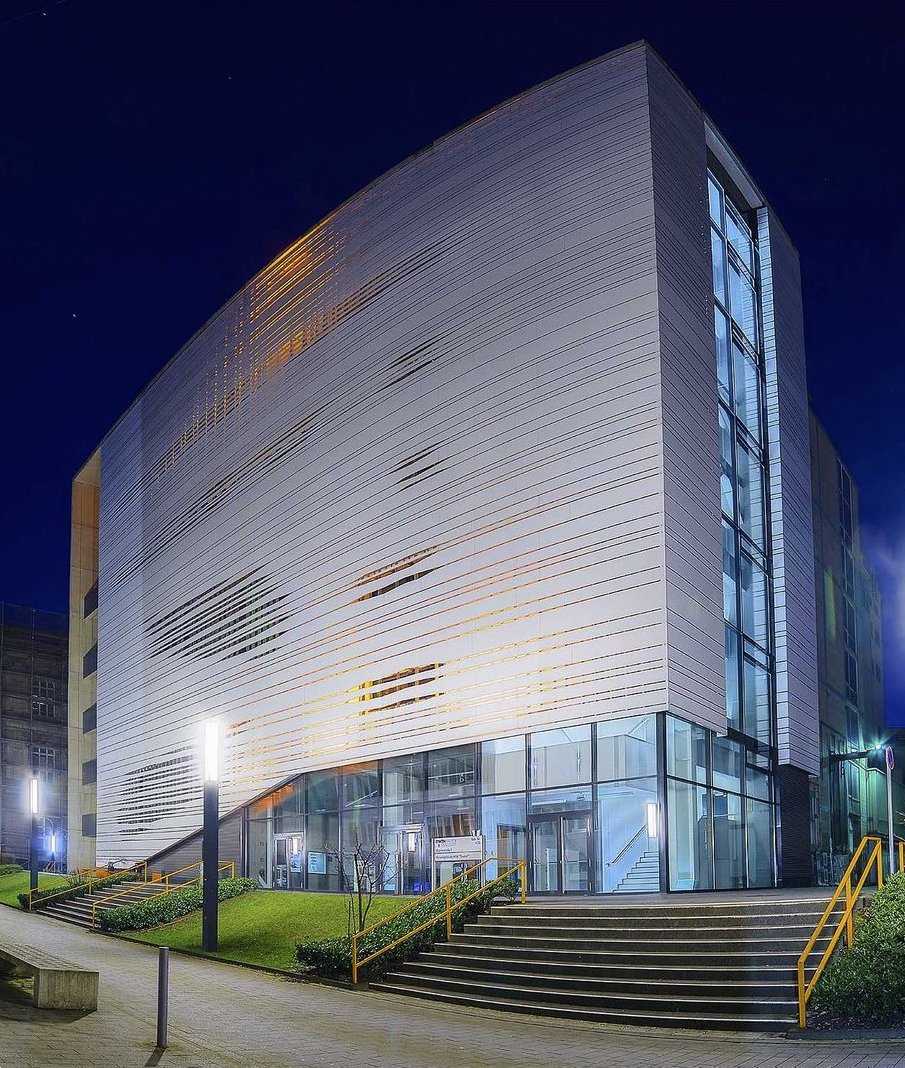
\includegraphics[width=0.9\textwidth]{toaster}
\end{center}
\end{column}

\begin{column}{0.5\textwidth}
\textbf{Theory}\vspace{0.2cm}
\begin{itemize}
\item Notation \vspace{0.2cm}
\item The Neural Tangent Kernel \vspace{0.2cm}
\item Theoretical Motivation
\end{itemize} \vspace{0.5cm}
\textbf{Practice}\vspace{0.2cm}
\begin{itemize}
\item Dynamic Linear Dimensionality Reduction (DLDR)  \vspace{0.2cm}
\item Projected SGD (P-SGD) \vspace{0.2cm}
\item Numerical Experiments  \vspace{0.2cm}
\end{itemize}
\end{column}

\end{columns}
\end{frame}

%%%%%%%%%%%%%%%%%%%%%%%%%%%%%%%%%%%%%%%%%%%%%%%%%%%%%%%%%%%%%%%

\section{Notation 1/2}
\begin{frame}
\begin{itemize}
\item We investigate a single output neural network
\[ f: \R^{n_0} \times \R^n \to \R : (x,w) \mapsto f(x,w). \]
\item In order to train the network we require a training set
\[ \X = \big \{ (x_i,y_i) \mid i=1, \dots, m \big \} \subset \R^{n_0} \times \R. \] 
\item Also, we require a differentiable loss function
\[ \ell: \R \times \R \to \R_+ : (x,y) \mapsto \ell(x,y). \]
\item Training the network is accomplished by minimizing the empirical error
\[ E : \R^n \to \R_+ : w \mapsto \sum_{i=1}^{m} \ell \big (f(x_i,w), y_i \big ). \]
\end{itemize}
\end{frame}



\section{Notation 2/2}
\begin{frame}
\begin{itemize}
\item The training dynamics are governed by the differential equation
\[ \partial_t w_t = -\nabla E (w_t ) = - \sum_{i=1}^{m} \nabla_w f(x_i,w_t) \cdot \nabla _x \ell \big ( f(x_i,w_t), y_i \big ). \]
\item Written in terms of vectors and matrices this is equivalent to
\[ \partial_tw_t = - \nabla_w f(\X, w_t)\tr \cdot \nabla_{f(\X,w_t)} E. \]
\item Here we used the notations
\[ \nabla_w f(\X, w_t)\tr := \Big [ \nabla_wf(x_1,w_t), \dots, \nabla_wf(x_m, w_t) \Big ] \in \R^{n \times m}, \]
\[ \nabla_{f(\X,w_t)} E := \Big [ \nabla_x \ell \big ( f(x_1,w_t), y_1 \big ), \dots, \nabla_x \ell \big ( f(x_m,w_t), y_m \big ) \Big ]\tr \in \R^m. \]
\end{itemize}
\end{frame}



\section{The Neural Tangent Kernel (NTK)}
\begin{frame}
\begin{itemize}
\item The Neural Tangent Kernel refers to the matrix
\[ \Theta_{w} = \nabla_wf(\X,w) \cdot \nabla_wf(\X,w)\tr. \]
\item According to [2], in the \textbf{infinite-width limit}, it holds that
\[ \nabla_wf(\X,w_t) \cdot \nabla_wf(\X,w_t)\tr = \Theta_{w_t} = \Theta_{w_0} = \nabla_wf(\X,w_0) \cdot \nabla_wf(\X,w_0)\tr. \] 
\item Using a singular value decomposition $\nabla_wf(\X,w_0) = U_0 \Sigma_0 V_0\tr$, yields
\[ \Theta_{w_0} = \nabla_wf(\X,w_0) \cdot \nabla_wf(\X,w_0)\tr  = U_0 \Sigma_0 \Sigma_0\tr  U_0\tr. \]
\item According to [3] and [4], the limiting NTK is low-rank, so $\Sigma_0$ is low-rank as well. \vspace{0.2cm}
\item Thus there exist $d \in \N$, $\tilde{U_0} := [e_1, \dots, e_d] \in \R^{m\times d}$, $\tilde{V_0} := [e_1, \dots, e_d] \in \R^{n\times d}$ and $\tilde{\Sigma}_0 = \text{diag}(\sigma_1, \dots, \sigma_d) \in \R^{d \times d}$ with
\[ \Sigma_0 \approx \tilde{U}_0 \tilde{\Sigma}_0 \tilde{V}_0\tr. \]
\end{itemize}
\end{frame}



\section{Theoretical Motivation}
\begin{frame}
\center{\fbox{Assumption: The layer width is unlimited.}} \vspace{1cm}
\begin{itemize}
\item Using the properties of the NTK, we derive
\[ \partial_tw_t = - \nabla_w f(\X, w_t)\tr \cdot \nabla_{f(\X,w_t)} E = - \nabla_w f(\X, w_0)\tr \cdot \nabla_{f(\X,w_t)} E. \]
\item Also, since the NTK is low-rank, we have
\[ \nabla_wf(\X,w_0) = U_0 \Sigma_0 V_0\tr \approx U_0 \tilde{U}_0 \tilde{\Sigma}_0 \tilde{V}_0\tr  V_0\tr . \]
\item As a consequence, the dynamics of gradient flow are approximately governed by
\[ \partial_t w_t = -\nabla_wf(\X,w_0)\tr  \cdot \nabla_{f(\X,w_t)} E \approx - V_0 \tilde{V}_0 \Big ( \tilde{\Sigma}_0 \tilde{U}_0\tr  U_0\tr  \cdot \nabla_{f(\X,w_t)} E \Big ). \]
\end{itemize}
\vspace{1cm}
$\Rightarrow$ The training dynamics $\partial_tw_t$ of dimension $n$ could be well embedded just in a $d$-dimensional space.
\end{frame}



\section{Illustration of the low-dimensional trajectory hypothesis}
\begin{frame}
\begin{columns}[c]

\begin{column}{0.5\textwidth}
\begin{center}
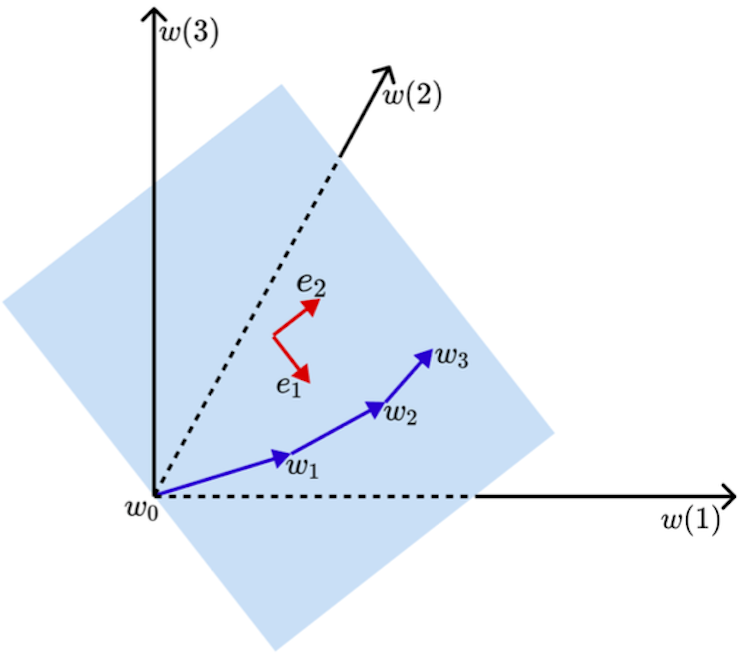
\includegraphics[width=0.99\textwidth]{approach.png}
\end{center}
\end{column}

\begin{column}{0.5\textwidth}
\begin{itemize}
\item $ V_0 \tilde{V}_0$ refers to the the orthonormal basis of the subspace \vspace{0.5cm}
\item $\tilde{\Sigma}_0 \tilde{U}_0\tr  U_0\tr  \cdot \nabla_{f(\X,w_t)} E$ describes the projected gradient 
\end{itemize}
\end{column}
\end{columns}
\vspace{0.5cm}
\[ \partial_t w_t = -\nabla E(w_t) = -\nabla_wf(\X,w_0)\tr  \cdot \nabla_{f(\X,w_t)} E \approx - V_0 \tilde{V}_0 \Big ( \tilde{\Sigma}_0 \tilde{U}_0\tr  U_0\tr  \cdot \nabla_{f(\X,w_t)} E \Big ) \]
\end{frame}



%\section{Dynamic Linear Dimensionality Reduction}

%\begin{frame}
%\center{\fbox{How to find the low-dimensional subspace?}} \vspace{1cm}
%\begin{itemize}
%\item 1) Sample $t$ steps of parameters during the training, namely, $\{w_1, w_2, \dots , w_t \}$. \vspace{0,2cm}
%\item 2) Centralize these as $\bar{w} = \frac{1}{t}\sum_{i=1}^{t} w_i$ and let $W = [ w_1 - \bar{w}, \dots, w_t - \bar{w}]$. \vspace{0,2cm}
%\item 3) Find a d-dimensional subspace spanned by $P = [e_1,e_2,\dots,e_d]$ to cover $W$. \vspace{1cm}
%\end{itemize}
%The third step is to find a subspace that the distance of $W$ and $P^TW$ is minimized. \vspace{1cm}
%\begin{itemize}
%\item We consider the SVD $W=U\Sigma V^T$ with $U = [u_1, \dots, u_n]$, $\Sigma = \text{diag}(\sigma_1, \dots, \sigma_t)$ and $V = [v_1, \dots, v_t]$. The first $d$ columns of $U$ are the independent variables. \vspace{0,2cm}
%\item Compute $v_i$ for $i=1, \dots, d$ by the spectral decomposition of $W^TW$ and derive
%\[ Wv_i = \sigma_iu_i, \quad i=1, \dots, d. \]
%\end{itemize}
%\end{frame}

\section{Agenda}
\begin{frame}
\begin{columns}[c]

\begin{column}{0.5\textwidth}
\begin{center}
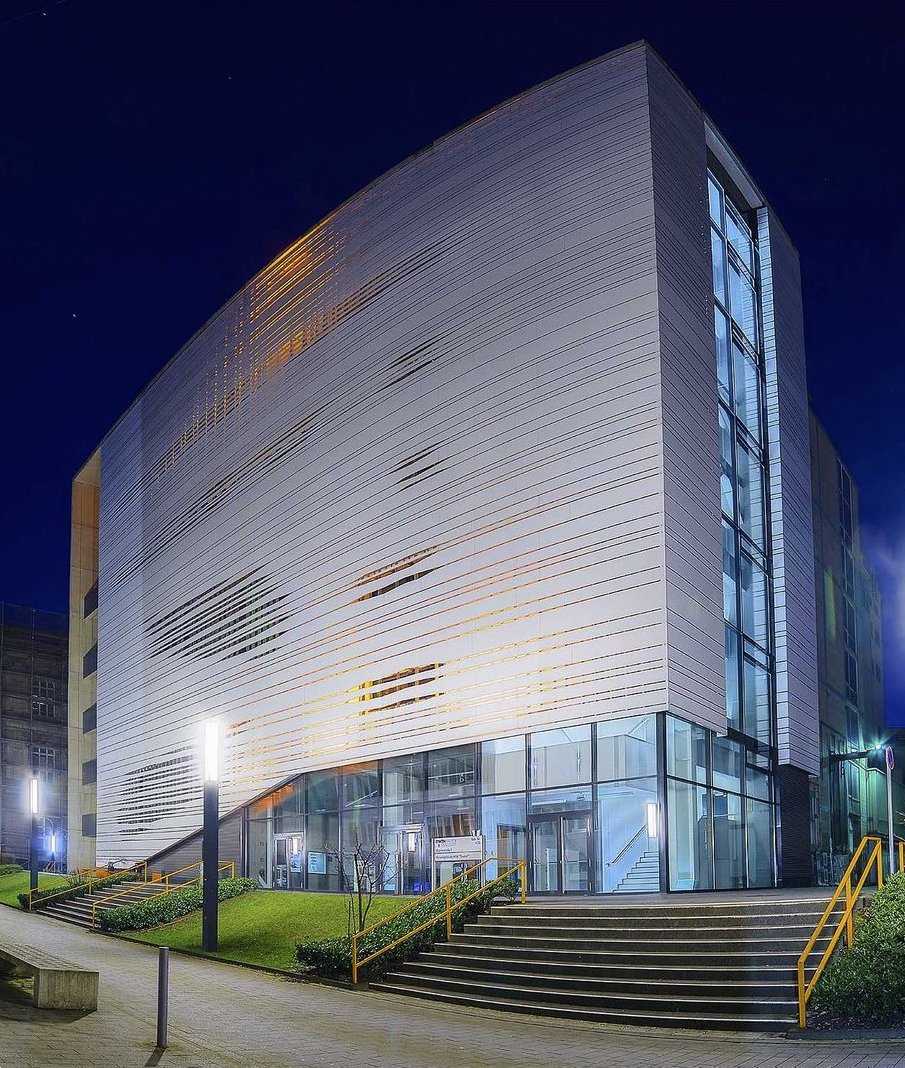
\includegraphics[width=0.9\textwidth]{toaster}
\end{center}
\end{column}

\begin{column}{0.5\textwidth}
\textbf{Theory}\vspace{0.2cm}
\begin{itemize}
\item Notation \vspace{0.2cm}
\item The Neural Tangent Kernel \vspace{0.2cm}
\item Theoretical Motivation
\end{itemize} \vspace{0.5cm}
\textbf{Practice}\vspace{0.2cm}
\begin{itemize}
\item Dynamic Linear Dimensionality Reduction (DLDR)  \vspace{0.2cm}
\item Projected SGD (P-SGD) \vspace{0.2cm}
\item Numerical Experiments  \vspace{0.2cm}
\end{itemize}
\end{column}

\end{columns}
\end{frame}


\section{Low-Dimensional Subspace Extraction}
\begin{frame}
\begin{figure}
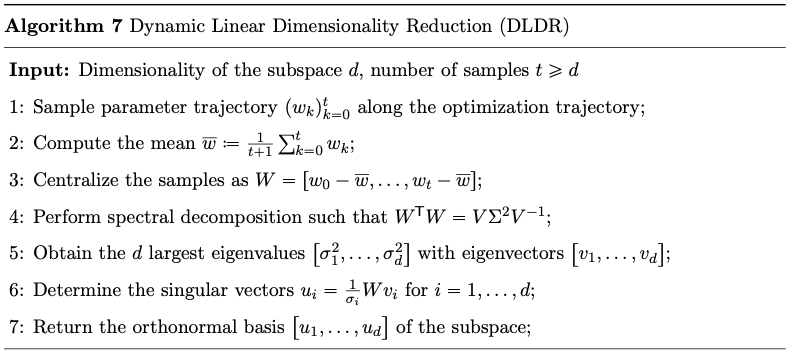
\includegraphics[width=\textwidth]{dldr.png}
\end{figure}
\end{frame}


\section{Training in Low-Dimensional Subspaces}
\begin{frame}
\begin{figure}
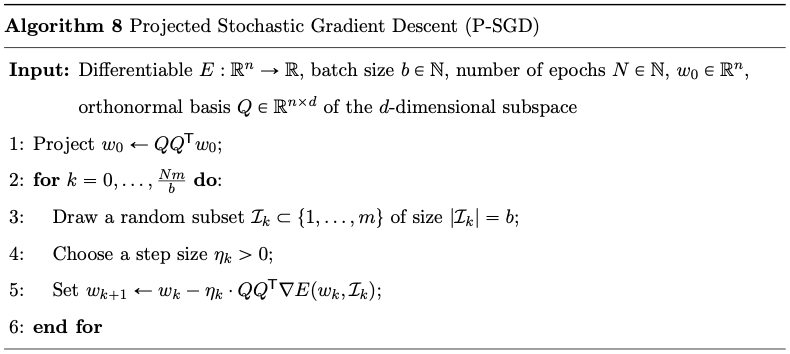
\includegraphics[width=\textwidth]{p-sgd}
\end{figure}
\end{frame}


\section{Optimizing ResNet8 in a 15-dimensional space can achieve comparable performance as regular training in the full parameter space.}
\begin{frame}
\begin{figure}
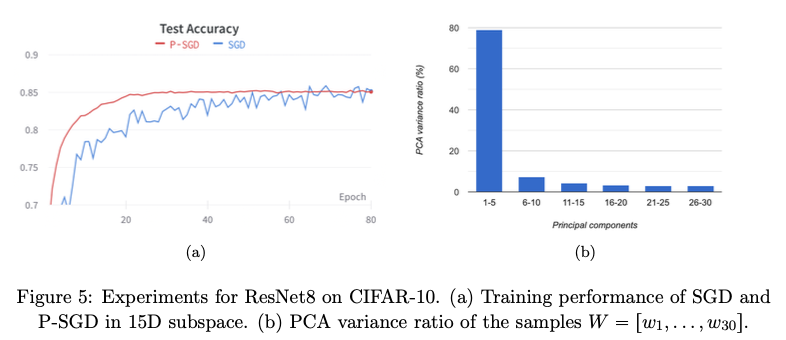
\includegraphics[width=0.99\textwidth]{exp-1}
\end{figure}
\end{frame}

\section{Optimizing DNNs in 40-dimensional spaces can achieve comparable performance as regular training in the full parameter space.}
\begin{frame}
\begin{figure}
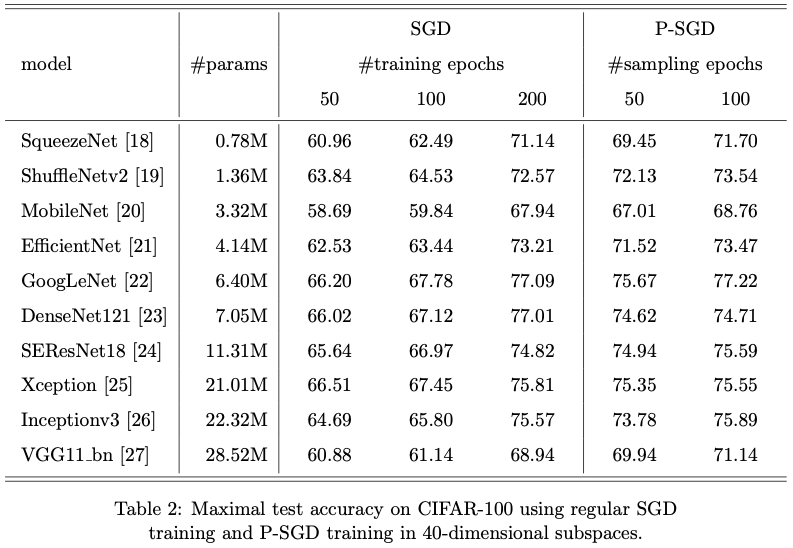
\includegraphics[width=0.8\textwidth]{exp-2}
\end{figure}
\end{frame}

\section{For the design of cost-efficient optimization algorithms, it is key to minimize the computational effort spent on sampling.}
\begin{frame}
\begin{figure}
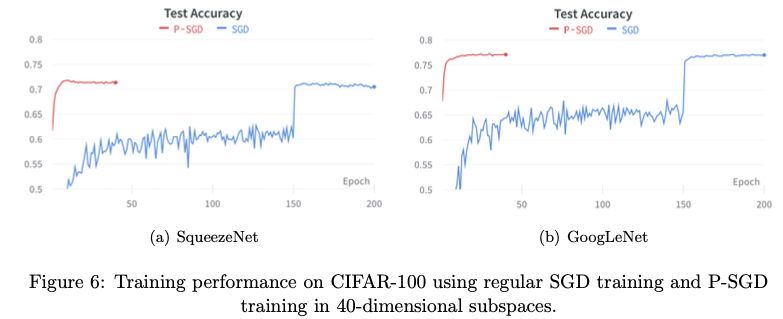
\includegraphics[width=0.99\textwidth]{exp-3-img}
\end{figure}
\end{frame}

\section{The complexity of generating samples far exceeds the complexity of performing PCA on these samples.}
\begin{frame}
\begin{figure}
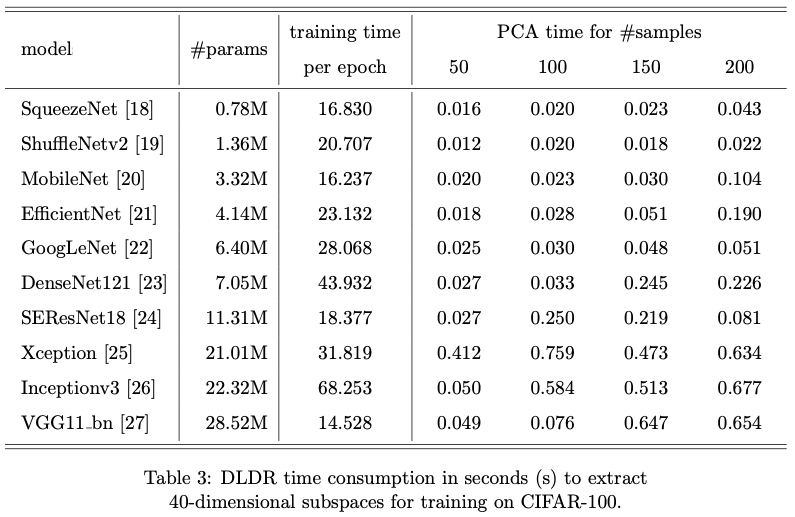
\includegraphics[width=0.85\textwidth]{exp-3}
\end{figure}
\end{frame}

\section{Extracting low-dimensional subspaces is associated with two problems}
\begin{frame}
\centering
\vspace{5cm}
Which strategy should be used for sampling? \\ \ \\
Which subspace dimension should be used for training?
\end{frame}

\section{Samples should be generated by taking the average over the parameters after each batch.}
\begin{frame}
\begin{figure}
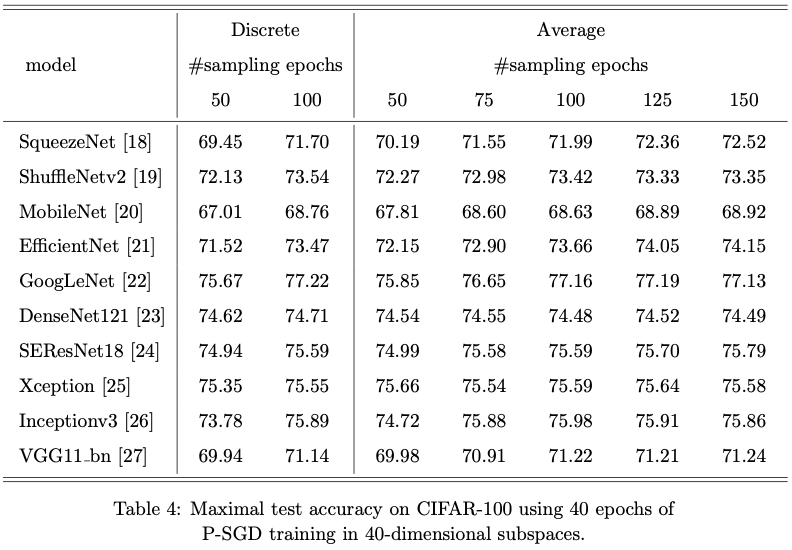
\includegraphics[width=0.8\textwidth]{exp-4}
\end{figure}
\end{frame}

\section{Samples should be generated once per epoch and the dimension can be chosen arbitrarily, as long as it is not too small.}
\begin{frame}
\begin{figure}
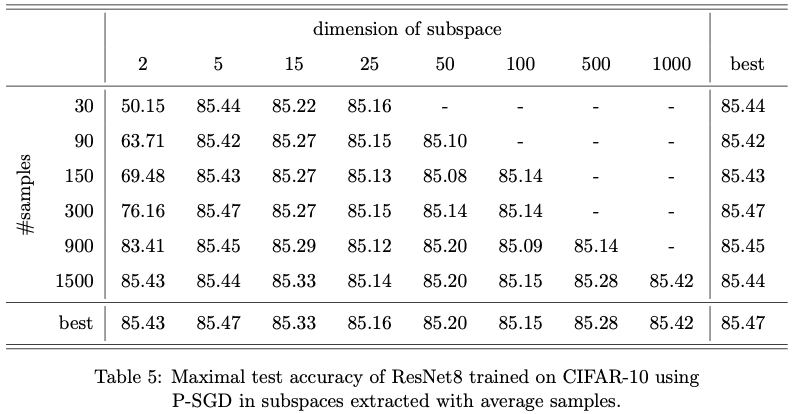
\includegraphics[width=0.99\textwidth]{exp-5}
\end{figure}
\end{frame}

\section{Possibilties for further work could include the design of cost-efficient low-dimensional training algorithms.}
\begin{frame}
\begin{itemize}
\item A future low-dimensional training algorithm could proceed as follows:  \vspace{0.5cm}
\begin{itemize}
\item []
\begin{itemize}
\item [1.] Generate samples by training in the full parameter space; \vspace{0.2cm}
\item [2.] While sampling, decide once enough examples have been generated; \vspace{0.2cm}
\item [3.] Extract a low-dimensional subspace based on these samples; \vspace{0.2cm}
\item [4.] Finish off the training by some final epochs of P-SGD in that space; \vspace{0.5cm}
\end{itemize}
\end{itemize}
\item \textbf{Major problem to solve:} Finding a criterium to decide once enough examples have been generated.
\end{itemize}
\end{frame}

\section{References}
\begin{frame}
\begin{itemize}
\item [{[1]}]  Tao Li, Lei Tan, Qinghua Tao, Yipeng Liu, Xiaolin Huang. \textit{Low Dimensional Trajectory Hypothesis is True: DNNs can be Trained in Tiny Subspaces}. IEEE Transactions on Pattern Analysis and Machine Intelligence, 2022. \\
\vspace{0.5cm}
\item [{[2]}] Arthur Jacot, Franck Gabriel, Cl\'{e}ment Hongler. \textit{Neural Tangent Kernel: Convergence and Generalization in Neural Networks}. Advances in Neural Information Processing Systems, volume 31, pages 8571-8580, 2018. \\
\vspace{0.5cm}
\item [{[3]}]  Zhou Fan, Zhichao Wang. \textit{Spectra of the Conjugate Kernel and Neural Tangent Kernel for Linear-Width Neural Networks}. Advances in Neural Information Processing Systems, volume 33, pages 7710-7721, 2020. \\
\vspace{0.5cm}
\item [{[4]}]  Amnon Geifman, Abhay Yadav, Yoni Kasten, Meirav Galun, David Jacobs, Ronen Basri. \textit{On the Similarity between the Laplace and Neural Tangent Kernels}. Advances in Neural Information Processing Systems, volume 33,  pages 1451-1461, 2020.
\end{itemize}
\end{frame}

%%%%%%%%%%%%%%%%%%%%%%%%%%%%%%%%%%%%%%%%%%%%%%%%%%%%%%%%%%%%%%%

\section{}

\begin{frame}

\begin{center}

\scalebox{1.5}{\textbf{Are there any questions?}} \\
\ \\


\includegraphics[width=0.95\textwidth]{ask}

\end{center}

\end{frame}

%%%%%%%%%%%%%%%%%%%%%%%%%%%%%%%%%%%%%%%%%%%%%%%%%%%%%%%%%%%%%%%

\end{document}
